\apendice{Especificación de diseño}\label{anex:C}

\section{Introducción}
Este apartado recoge el porqué de las decisiones finales que se han tomado acerca del diseño del software desarrollado, dividido en el diseño de datos, diseño arquitectónico y diseño de la interfaz de usuario.

\section{Diseño de datos}\label{sec:C_2}
El diseño de los datos es el diseño que tienen las entidades. Al no disponer de una base de datos, las entidades que se gestionan son clases Java.

Las clases más importantes a la hora de definir los datos que trabaja la aplicación están definidas en el paquete \ruta{datamodel}, estás son:
\begin{itemize}
	\item \ruta{Repository}. Sirve como definición de los datos que se obtienen de un repositorio de GitLab. Estos datos son:
	\begin{itemize}
		\item URL, nombre e ID del proyecto
		\item Métricas internas (\ruta{RepositoryInternalMetrics}). Representan los valores de los que se obtienen las métricas externas y que interesan para satisfacer los requisitos funcionales de la aplicación.
		\item Resultados de las métricas (\ruta{MetricsResults}). Al añadir un repositorio se espera que se calculen las métricas. Estas serán almacenadas aquí.
		\item Evaluación del proyecto (\textit{projectEvaluation}). Sirve como indicador del estado del proceso del proyecto, se espera almacenar el porcentaje de métricas evaluadas como `buenas' para el proyecto cada vez que se añadan unos nuevos resultados de métricas.
		\item Se ha definido la igualdad de los repositorios por su URL, ID y nombre.
	\end{itemize}
	\item \ruta{RepositoryInternalMetrics}. Sirve para separar lo que define a un proyecto de los datos que se necesitan para calcular las métricas. Contiene: la fecha de medición, el número total de issues, el número total de commits, el número de issues cerradas, una colección de días que se tardan en cerrar las issues, otra colección con las fechas de los commits, y el tiempo de vida del proyecto. Se define el método \textit{equals} a partir de la fecha de medición.
	\item \ruta{User}. Sirve para almacenar información que se obtiene de GitLab acerca del usuario que ha iniciado sesión: el ID de usuario, la URL del avatar, el e-mail, el nombre y el nombre de usuario.
\end{itemize}

%\section{Diseño procedimental}

\section{Diseño arquitectónico}
En este apartado se describen las clases y la estructura de los paquetes de los que consta el proyecto software.

\subsection{Paquete repositorydatasource}
El paquete define el framework de conexión a una forja de repositorios e implementa la conexión a GitLab.

\imagen{AnexC_RepositoryDataSource}{Paquete reposutorydatasource}

Para crear un \textit{Repositorydatasource} con acceso a otra forja solo se tiene que implementar las dos interfaces, sin necesidad de hacer más cambios en el código.

\subsection{Paquete metricsengine}
El paquete define el framework de medición y sigue el diseño descrito en \textit{Soporte de Métricas con Independencia del Lenguaje para la Inferencia de Refactorizaciones} \citep{marticorena_sanchez_soporte_2005}, con unos pequeños cambios:

\begin{itemize}
	\tightlist
	\item Se ha aplicado a las métricas concretas el patrón \textit{\textbf{Singleton}} \footnote{\url{https://refactoring.guru/design-patterns/singleton}}, que obliga a que solo haya una única instancia de cada métrica; y se ha aplicado el patrón \textit{\textbf{Método fábrica}} \footnote{\url{https://refactoring.guru/design-patterns/factory-method}} tal y como se muestra en la Fig. \ref{fig:M3_CambiosFrameworkMedicion1}, de forma que \textit{MetricConfiguration} no esté asociada con la métrica en sí, sino con una forma de obtenerla.\\
	La intencionalidad de esto es facilitar la persistencia de un perfil de métricas. Las métricas se podrían ver como clases estáticas, no varían en tiempo de ejecución y solo debería haber una instancia de cada una de ellas. Por ello, al importar o exportar un perfil de métricas con su conjunto de configuraciones de métricas, estas configuraciones no deberían asociarse a la métrica, sino a la forma de acceder a la única instancia de esa métrica. 
	\item Se han añadido los métodos \textit{evaluate} y \textit{getEvaluationFunction} en la interfaz \textit{IMetric}, ver Fig. \ref{fig:M3_CambiosFrameworkMedicion2}.\\
	Esto permitirá interpretar y evaluar los valores medidos sobre los valores límite de la métrica o configuración de métrica. Por ejemplo, puede que para unas métricas un valor aceptable esté comprendido entre el valor límite superior y el valor límite inferior; y para otras un valor aceptable es aquel que supere el límite inferior.\\
	\textit{EvaluationFunction} es una interfaz funcional \footnote{Enlaces a la documentación: \url{https://docs.oracle.com/javase/8/docs/api/java/lang/FunctionalInterface.html} --- \url{https://docs.oracle.com/javase/8/docs/api/java/util/function/package-summary.html}} 
	de tipo `\textit{función}': recibe uno o más parámetros y devuelve un resultado. Este tipo de interfaces son posibles a partir de la versión 1.8 de Java.\\
	Esto permite definir los tipos de los parámetros y de retorno de una función que se puede almacenar en una variable. De este modo se puede almacenar en una variable la forma en la que se puede evaluar la métrica.
\end{itemize}

\imagen{M3_CambiosFrameworkMedicion1}{Patrones ``singleton'' y ``método fábrica'' sobre el framework de medición}

\imagen{M3_CambiosFrameworkMedicion2}{Añadido al framework de medición la evaluación de métricas}

\subsection{Paquete gui}
En este paquete se ha definido toda la interfaz gráfica.




\subsection{Paquete exceptions}
En este paquete se han definido las excepciones de la aplicación, además se han trabajan con códigos de error y mensajes para poder ser identificados y comprendidos en el logger fácilmente. Se ha creado un diseño en el que, para definir nuevas excepciones, se puede extender de \textit{ApplicationException}, copiar y adaptar los constructores y modificar con \textit{@Override} el método \textit{generateMessage()} con los mensajes personalizados en un \textit{switch} para cada código de error:

\begin{figure}[!h]
	\centering
	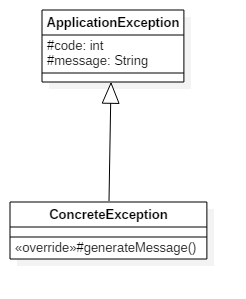
\includegraphics[width=0.5\textwidth]{AnexC_Exceptions}
	\caption{Paquete exceptions}\label{fig:AnexC_Exceptions}
\end{figure}
\FloatBarrier

\subsection{Paquete datamodel}
El paquete datamodel contiene las tres clases que se han descrito anteriormente en la sección \ref{sec:C_2}.

\subsection{Paquete app}
Contiene las clases que integran todos los módulos y sirve de conexión entre la interfaz de usuario y la parte lógica de la aplicación.

\begin{figure}[!h]
	\centering
	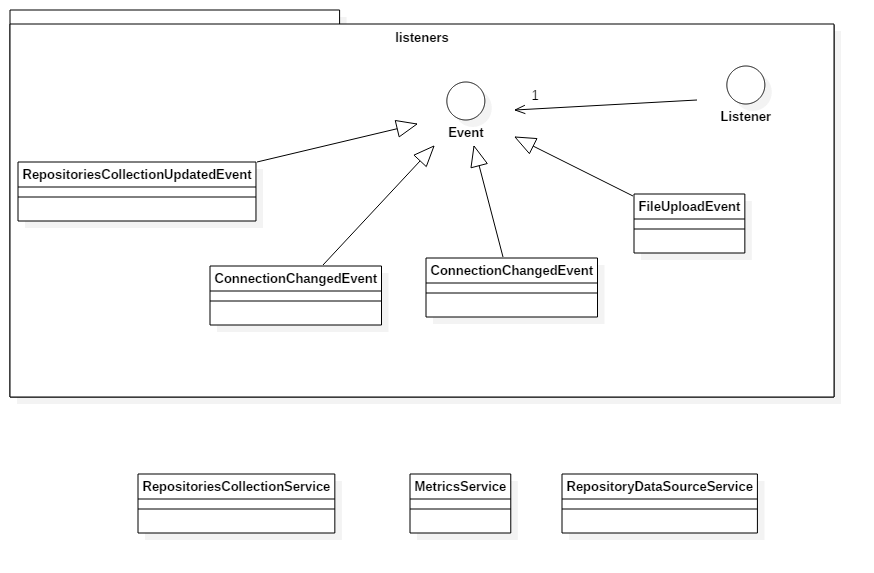
\includegraphics[width=0.5\textwidth]{AnexC_app}
	\caption{Paquete app}\label{fig:AnexC_app}
\end{figure}
\FloatBarrier

\begin{description}
	\item[MetricsService] Define una fachada de conexión entre el motor de métricas y el resto de componentes.
	\item[RepositoriesCollectionService] Se encarga de almacenar los repositorios en una colección
	\item[RepositoriesCollectionService] Define una fachada entre la fuente de datos (\textit{repositorydatasource}) y el resto de componentes.
\end{description}

También cuenta con un paquete para el patrón observador. En este se definen la interfaz \textit{Listener} y la interfaz \textit{Event}, y se implementan algunos eventos. La interfaz \textit{Event} sirve para implementar eventos a partir de ella, estos eventos normalmente tienen información relativa al suceso que ocurre. Por ejemplo, \textit{CurrentMetricProfileChangedEvent} contiene información sobre un cambio de perfil de métricas: el viejo perfil y el nuevo. La interfaz \textit{Listener} define una función a la que se le pasa un evento y sirve como interfaz funcional para ejecutar una acción (función lambda) que recibe por parámetro el evento.
